\documentclass[border=5pt]{standalone}
\usepackage{tikz}
\usepackage{amsmath}
\begin{document}
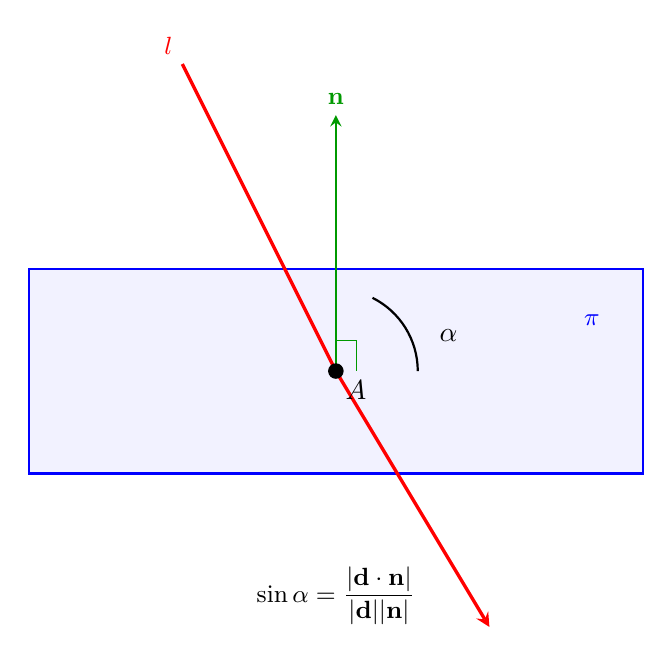
\begin{tikzpicture}[scale=1.3, >=stealth]
  % Angle between line and plane

  % Plane
  \fill[blue!10, opacity=0.5] (-3,-1) -- (3,-1) -- (3,1) -- (-3,1) -- cycle;
  \draw[thick, blue] (-3,-1) -- (3,-1) -- (3,1) -- (-3,1) -- cycle;
  \node[blue, font=\small] at (2.5, 0.5) {$\pi$};

  % Line intersecting plane
  \draw[very thick, red, ->] (-1.5, 3) -- (0, 0) -- (1.5, -2.5);
  \node[red, font=\small, above left] at (-1.5, 3) {$l$};

  % Normal vector
  \draw[->, thick, green!60!black] (0, 0) -- (0, 2.5) node[above, font=\small] {$\mathbf{n}$};

  % Angle between line and plane
  \draw[thick] (0.8, 0) arc (0:{atan2(3,1.5)}:0.8);
  \node at (1.1, 0.35) {$\alpha$};

  % Right angle for normal
  \draw[green!60!black, thin] (0, 0.3) -- (0.2, 0.3) -- (0.2, 0);

  % Point of intersection
  \filldraw[black] (0, 0) circle (2pt) node[below right] {$A$};

  % Formula
  \node[font=\small] at (0, -2.2) {$\sin\alpha = \dfrac{|\mathbf{d}\cdot\mathbf{n}|}{|\mathbf{d}||\mathbf{n}|}$};
\end{tikzpicture}
\end{document}
